% BlackboxNLP 2026 Reproducibility Challenge submission (Special Track)
% Build: ./prepare_tables.sh && pdflatex main && bibtex main && pdflatex main && pdflatex main
% Track limit: max 6 pages + references (verified against
% https://blackboxnlp.github.io/2026/call on 2026-07-18); double-blind.
% Tables T1-T4 are \input from paper/generated/, which prepare_tables.sh
% copies from ../analysis/tables/ (generated by analysis/make_tables.py),
% promoting {table} to {table*}. Figures come from ../analysis/figures/.
% Do not retype numbers here -- regenerate the artifacts instead.
\documentclass[11pt]{article}
\usepackage[review]{acl}   % review mode = anonymized; switch to [final] for camera-ready
\usepackage{times,latexsym,graphicx,booktabs,amsmath}
\graphicspath{{../analysis/figures/}}

\title{Do Function Vectors Transfer? A Reproducibility Study on Modern GQA Language Models}
\author{Anonymous BlackboxNLP submission}

\begin{document}
\maketitle

\begin{abstract}
Function vectors \citep[FVs;][]{todd2024function} are compact task
representations formed by summing the task-conditioned outputs of a small set
of attention heads; added to the residual stream, they induce zero-shot task
execution. We first reproduce the core FV results on GPT-J-6B --- our antonym
accuracy at the paper's operating layer is 49.2\% against a reported
$48.2 \pm 2.0\%$ --- and then stress-test the method's \emph{generalizability}
on three modern grouped-query-attention models: Llama-3.1-8B, Qwen2.5-7B, and
Mistral-7B-v0.3. The core mechanism transfers: at the paper's GPT-J
operating point (top-10 heads), FVs raise zero-shot accuracy by $+0.33$ to
$+0.94$ on 4 of 6 tasks for Llama-3.1 and 5 of 6 for Qwen2.5. The paper's
heuristics and interpretive claims, however, prove GPT-J-specific in five
ways. The optimal injection layer drifts from ${\sim}0.32\times$ depth (the
source of the ``inject at $L/3$'' rule) to ${\sim}0.61\times$ depth on
Qwen2.5, and no single head count is optimal across models and tasks.
English--French translation fails on all three modern models.
Mistral-7B-v0.3 shows near-zero FV effect at top-10 heads on every task,
recovering monotonically with head count (accuracy 0.45 at $k{=}100$) ---
consistent with a more distributed task representation, and mirrored by the
flattest measured concentration of causal effect. Finally, FV vocabulary
decodability does not generalize: the antonym FV decodes to task-relevant
tokens on GPT-J, but on the modern models even working FVs decode to noise.
We report these negative results as boundary conditions that sharpen,
rather than overturn, the function-vector
picture.\footnote{An anonymized mirror of the code, the modernization
patch, and all raw result files is available at
\url{https://anonymous.4open.science/r/REPLACE-ME}; a de-anonymized
release will accompany publication.
% TODO-CHECK(user): paste the real anonymous.4open.science URL over
% REPLACE-ME before submission.
}
\end{abstract}

\section{Introduction}

Mechanistic interpretability findings are typically established on a small
number of models and then quoted as if they were properties of transformer
language models in general. Whether they actually are is an empirical
question, and an increasingly pressing one: the open-weight models in wide
use today differ from the 2023-era models on which many influential results
were obtained --- grouped-query attention \citep[GQA;][]{ainslie2023gqa},
much larger vocabularies, different tokenizers, and different training data
and scale.

We stress-test one such result along this axis. \citet{todd2024function}
showed that a small set of attention heads carries a compact, causally
efficacious representation of an in-context task: summing those heads'
task-conditioned outputs yields a \emph{function vector} (FV) that, added to
a hidden state at an early-middle layer, makes the model perform the task
zero-shot. The finding comes with practical heuristics --- select the top
heads by average indirect effect (10 for GPT-J, scaled up with a model's
head count), inject around one third of network depth --- and an
interpretive claim (FVs decode to task-relevant vocabulary for most tasks)
that subsequent work tends to adopt wholesale.

Following the reproducibility-challenge theme of \emph{generalizability}, we
ask: do the FV findings, the heuristics, and the interpretation survive the
move to modern GQA models? We reproduce the original pipeline on GPT-J-6B
\citep{wang2021gptj} as an anchor, then run it unchanged (up to dtype and
GQA dispatch) on Llama-3.1-8B \citep{grattafiori2024llama3}, Qwen2.5-7B
\citep{qwen2025qwen25}, and Mistral-7B-v0.3 \citep{jiang2023mistral}, across
the six headline tasks of the original paper.

Our findings, in brief: (1)~the reproduction succeeds --- GPT-J numbers
match the paper; (2)~the core claim generalizes --- FVs induce large
zero-shot effects on Llama-3.1 (4/6 tasks) and Qwen2.5 (5/6); (3)~the
heuristics do not --- the optimal injection layer drifts substantially later
in depth fraction on newer models, and the best head count varies by model
and task; (4)~there are sharp boundary conditions --- English--French fails
on all three modern models, present-tense-to-past fails only on Llama-3.1,
and Mistral-7B-v0.3 is a systematic null at top-10 heads whose effect
recovers monotonically as heads are added; (5)~the interpretability
narrative that FVs decode to task vocabulary is itself GPT-J-specific ---
modern models' FVs work without being decodable. We intend these results in
the spirit of the challenge: they enrich the original work by mapping where
its findings hold, where they bend, and where they break.

\section{Background: Function Vectors}

We summarize the method of \citet{todd2024function}; notation follows their
paper. A task $t$ (e.g.\ antonym) is presented as 10-shot in-context prompts
$p^t_i$ of word pairs. For each attention head $(\ell, j)$ (layer $\ell$,
head index $j$), the \emph{task-conditioned mean activation} is the head's
output averaged over a set of prompts $P_t$:
$\bar{a}^t_{\ell j} = \tfrac{1}{|P_t|}\sum_{p \in P_t} a_{\ell j}(p)$.

Heads are ranked by causal mediation
\citep{pearl2001direct,vig2020investigating}: on \emph{corrupted} prompts
$\tilde{p}^t_i$ with shuffled labels (destroying the input--output mapping
while preserving the domain), the head's activation is patched to
$\bar{a}^t_{\ell j}$ and the resulting increase in probability of the
correct answer is the causal indirect effect; averaging over prompts and
tasks gives the \emph{average indirect effect} (AIE). The FV is the sum of
mean activations over the set $\mathcal{A}$ of top-AIE heads,
$v_t = \sum_{(\ell,j)\in\mathcal{A}} \bar{a}^t_{\ell j}$. Their footnote~1
prescribes $|\mathcal{A}| = 10$ for GPT-J, scaled approximately
proportionally to a model's attention-head count for larger models (20 for
Llama-2-7B, 50 for Llama-2-13B and GPT-NeoX, 100 for Llama-2-70B). At
inference, $v_t$ is simply added to the hidden state at one layer $\ell$ of
the residual stream.

On GPT-J, \citet{todd2024function} report that adding the FV at layer 9
(${\approx}L/3$ of 28 layers) raises zero-shot accuracy, macro-averaged over
the six headline tasks, from $5.5 \pm 0.8\%$ to $57.5 \pm 1.7\%$, with
strong causal effects concentrated at early-middle layers, and that FVs
also repair shuffled-label 10-shot prompts ($39.1 \pm 1.2\%$ to
$90.8 \pm 0.9\%$). They further show that decoding an FV through the
unembedding yields tokens in the task's output space for most tasks
(their \S3.2). The mechanism is related to,
but distinct from, the contemporaneous task vectors of
\citet{hendel2023incontext}, which use a single hidden state rather than a
sum of selected head outputs.

\section{Experimental Setup}

\paragraph{Models.} GPT-J-6B (28 layers, multi-head attention, the
reproduction anchor) and three modern GQA models: Llama-3.1-8B (32 layers),
Qwen2.5-7B (28), Mistral-7B-v0.3 (32).\footnote{Checkpoint
\texttt{mistralai/Mistral-7B-v0.3}; \citet{jiang2023mistral} describes
v0.1 --- v0.3 differs, i.a., in tokenizer and vocabulary size.} All are
base (non-instruct) checkpoints. All four satisfy
$d_{\text{head}} \times n_{\text{heads}} = d_{\text{model}}$, which the
original codebase assumes when splitting the attention output projection
input into per-head contributions.

\paragraph{Tasks.} The six headline tasks of the original paper: antonym,
capitalize, country-capital, english-french, present-past, singular-plural,
using the original dataset files.

\paragraph{Held fixed.} Everything the original pipeline specifies: the
authors' code and prompt format (\texttt{Q:}/\texttt{A:}), seed (42),
\texttt{transformers} 4.49.0 (the authors' pin), 100 prompts for mean
activations, 25 shuffled-label trials for AIE, 10-shot prompts, top-10 heads
as the default operating point (the paper's GPT-J setting;
\S\ref{sec:heads} varies $k$ up to 100), and the evaluation protocol: test items are
filtered to those the model answers correctly with 10 clean shots (filtered
$n$ per task and model ranges from 41 to 819), and accuracy is first-token
top-1.

\paragraph{Changed.} Three deliberate changes and one constraint.
(i)~Modern models load in bfloat16 (GPT-J keeps the repository-default
fp32). (ii)~Model-architecture dispatch entries were added so Qwen2.5 and
Mistral route to the correct module names for hooking and editing the
attention output projection (\texttt{o\_proj}, a bias-free
\texttt{nn.Linear}, as in Llama). (iii)~An assertion enforcing
$d_{\text{head}} \times n_{\text{heads}} = d_{\text{model}}$ was added to
the per-head splitting code. This constraint \emph{excludes} the
Gemma-2/3 family \citep{gemmateam2024gemma2}, whose decoupled head
dimension violates it --- an architectural boundary condition of the
released FV tooling itself, prior to any empirical question.

\paragraph{Two dispatch bugs, disclosed.} Our first Qwen/Mistral runs
silently fell through two architecture-dispatch sites in the original
utilities (the intervention's output-projection hook and the FV assembly's
\texttt{out\_proj} resolution), because those sites enumerate model families
explicitly. Both were caught by cross-model sanity checks, fixed, and the
affected runs recomputed from cached activations; GPT-J and Llama runs never
hit these code paths. We flag this because silent dispatch fall-through is a
generic hazard when porting interpretability tooling to new architectures.

\paragraph{Metric.} Our headline quantity is the \emph{FV effect}
$\Delta = \text{acc}(\text{zero-shot} + \text{FV}) -
\text{acc}(\text{zero-shot})$, top-1, at the best-effect injection layer
$\ell^*$ (chosen per model--task by sweeping all layers). Raw with-FV
accuracy alone would flatter tasks with nontrivial zero-shot baselines
(e.g.\ singular-plural is 0.415 zero-shot on Mistral).
Table~\ref{tab:T1_gptj_reproduction} reports percentages; later tables
report fractions. Compute: one RTX~A6000, ${\sim}17.5$ GPU-hours total,
single run per cell.

\begin{table}[t]
\centering
\small
\begin{tabular}{lrrrrr}
\toprule
Task & Paper +FV (\%) & Ours +FV (\%) & Best layer & No-interv (\%) & FV effect (pp) \\
\midrule
antonym & 48.2±2.0 & 60.5 & L11 & 0.9 & +59.6 \\
capitalize & 70.5±2.4 & 77.5 & L10 & 0.0 & +77.5 \\
country-capital & 83.2±2.7 & 90.2 & L8 & 4.9 & +85.4 \\
english-french & 44.7±1.2 & 72.5 & L5 & 1.5 & +71.0 \\
present-past & 19.7±5.9 & 55.2 & L3 & 1.7 & +53.4 \\
singular-plural & 47.0±3.4 & 83.3 & L13 & 21.4 & +61.9 \\
\bottomrule
\end{tabular}
\caption{T1: GPT-J-6B reproduction. Paper values are Todd et al. Table 10 (zero-shot accuracy with the task FV at their chosen layer, mean±std over seeds); ours are best-over-layer-sweep (single seed 42), so ours upper-bound the paper protocol.}
\label{tab:T1_gptj_reproduction}
\end{table}

\begin{table}[t]
\centering
\small
\begin{tabular}{lrrrr}
\toprule
Task & GPT-J-6B & Llama-3.1-8B & Qwen2.5-7B & Mistral-7B-v0.3 \\
\midrule
antonym & +0.60 (L11) & +0.47 (L13) & +0.64 (L16) & +0.07 (L14) \\
capitalize & +0.78 (L10) & +0.88 (L14) & +0.94 (L17) & +0.01 (L20) \\
country-capital & +0.85 (L8) & +0.43 (L14) & +0.33 (L19) & +0.00 (L0) \\
english-french & +0.71 (L5) & +0.05 (L11) & +0.03 (L17) & +0.00 (L8) \\
present-past & +0.53 (L3) & +0.02 (L8) & +0.47 (L19) & +0.00 (L12) \\
singular-plural & +0.62 (L13) & +0.78 (L12) & +0.88 (L17) & +0.00 (L14) \\
tasks transferring (effect$>$0.3) & 6/6 & 4/6 & 5/6 & 0/6 \\
\bottomrule
\end{tabular}
\caption{T2: Zero-shot FV effect (accuracy with FV minus no-intervention accuracy, top-1) at the best-effect layer, per model and task.}
\label{tab:T2_generalization}
\end{table}


\section{Results}

\subsection{Reproduction on GPT-J}
\label{sec:repro}

Table~\ref{tab:T1_gptj_reproduction} shows the anchor run. All six tasks
reproduce a large FV effect ($+53.4$ to $+85.4$ points over a near-floor
zero-shot baseline). Our per-task with-FV accuracies all exceed the paper's
reported values, as expected from the protocol difference the caption
notes: we report the best layer over a sweep, which upper-bounds the
paper's fixed-layer protocol. The direct apples-to-apples check: injecting
at the paper's operating layer (layer 9), our antonym accuracy is
\textbf{49.2\%} against the reported $48.2 \pm 2.0\%$
\citep{todd2024function} --- within noise. On shuffled-label 10-shot
prompts, the antonym FV at the same layer lifts accuracy from 46.4\% to
85.9\%, matching the reported regime (six-task average $90.8 \pm 0.9\%$).
We conclude the pipeline is faithful.

\subsection{Generalization to modern models}
\label{sec:gen}

Table~\ref{tab:T2_generalization} is the headline result. At the paper's
GPT-J operating point, FVs transfer strongly to Llama-3.1-8B (4/6 tasks, effects
$+0.43$ to $+0.88$) and Qwen2.5-7B (5/6 tasks, $+0.33$ to $+0.94$), in
several cases exceeding the GPT-J effect (capitalize, singular-plural).
Grouped-query attention per se does not break function vectors.

The failures are patterned, not random. \textbf{english-french} fails on
\emph{all three} modern models ($+0.05$, $+0.03$, $+0.00$) while succeeding
on GPT-J ($+0.71$) --- a task-general boundary. \textbf{present-past} fails
\emph{only} on Llama-3.1 ($+0.02$ vs.\ $+0.53$ on GPT-J and $+0.47$ on
Qwen2.5) --- a model-specific one; notably singular-plural, an equally
morphological task, transfers on Llama-3.1 at $+0.78$, so ``morphology
fails'' is not the explanation. \textbf{Mistral-7B-v0.3} is a systematic
null at this operating point: $\Delta \le +0.07$ on every task. We return
to all three in \S\ref{sec:discussion}.

\begin{figure}[t]
\centering
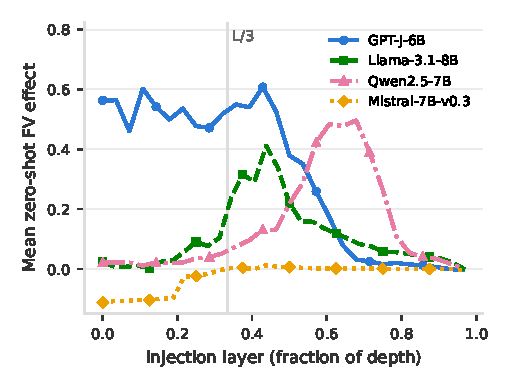
\includegraphics[width=\columnwidth]{F1_layer_sweep.pdf}
\caption{FV effect vs.\ injection depth, averaged over the six tasks
(top-10 heads; per-task curves in Appendix Figure~\ref{fig:f1b}). The
vertical line marks the $L/3$ heuristic of \citet{todd2024function}. The
effective band contains $L/3$ for GPT-J, sits slightly later for
Llama-3.1-8B, and at roughly $0.6\times$ depth for Qwen2.5-7B;
Mistral-7B-v0.3 shows no effective band, only early-layer degradation.}
\label{fig:f1}
\end{figure}

\subsection{Where should the FV be injected?}
\label{sec:layers}

Figure~\ref{fig:f1} shows the layer sweeps. GPT-J reproduces the original
picture: a broad effective band over the first half of the network that
includes $L/3$, collapsing to zero past mid-depth. On the modern models the
band \emph{narrows and drifts later}. Taking each model's tasks with
$\Delta > 0.3$ (best layers in Table~\ref{tab:T2_generalization}), the
median best-effect depth fraction is \textbf{0.32} on GPT-J (range
0.11--0.46), \textbf{0.42} on Llama-3.1 (0.38--0.44), and \textbf{0.61} on
Qwen2.5 (0.57--0.68). Injecting at the literal $L/3$ on Qwen2.5 (layer 9 of
28) would land \emph{outside} the effective band on every task and forfeit
most of the effect.

The practical upshot: ``inject at ${\sim}L/3$'' is a GPT-J-calibrated
heuristic, not a transformer-general law. The transferable finding is
weaker but still useful --- a contiguous effective band exists somewhere in
the first two thirds of depth and is cheap to locate with a sweep; its
location must be re-estimated per model.

\begin{table}[t]
\centering
\small
\begin{tabular}{lrrrrrrr}
\toprule
Model & Task & Layer & k=5 & k=10 & k=20 & k=50 & k=100 \\
\midrule
GPT-J-6B & antonym & L11 & 0.55 & 0.61 & 0.70 & 0.64 & -- \\
GPT-J-6B & country-capital & L8 & 0.73 & 0.90 & 0.93 & 0.93 & -- \\
Llama-3.1-8B & antonym & L13 & 0.58 & 0.48 & 0.69 & 0.73 & -- \\
Llama-3.1-8B & country-capital & L14 & 0.12 & 0.48 & 0.29 & 0.93 & -- \\
Qwen2.5-7B & antonym & L16 & 0.43 & 0.64 & 0.62 & 0.50 & -- \\
Qwen2.5-7B & country-capital & L19 & 0.31 & 0.38 & 0.81 & 0.93 & -- \\
Mistral-7B-v0.3 & antonym & L14 & 0.09 & 0.12 & 0.16 & 0.34 & 0.45 \\
Mistral-7B-v0.3 & country-capital & L0 & 0.05 & 0.05 & 0.00 & 0.05 & -- \\
\bottomrule
\end{tabular}
\caption{T3: Zero-shot accuracy with FV built from top-k heads, injected at the best layer from the main (k=10) sweep. k=100 run for Mistral antonym only; dashes = not run.}
\label{tab:T3_k_ablation}
\end{table}


\subsection{How many heads?}
\label{sec:heads}

Table~\ref{tab:T3_k_ablation} varies the number of summed heads $k$ at each
cell's fixed best layer, reporting raw with-FV accuracy. Two observations.
First, top-10 is not a universal operating point: on GPT-J antonym the
accuracy keeps rising to $k{=}20$ (0.70); on Llama-3.1 country-capital,
$k{=}10$ (0.48) is far from $k{=}50$ (0.93); on Qwen2.5 antonym, $k{=}10$
is already the peak (0.64). The $k$-response is model- \emph{and}
task-dependent. Under the original paper's own proportional-scaling
guidance (${\sim}20$ heads for these 28--32-head models, vs.\ GPT-J's 16),
the conclusion is unchanged: at $k{=}20$ Mistral antonym remains near
floor (0.16) while Llama-3.1 (0.69) and Qwen2.5 (0.62) transfer. (Mistral
country-capital had no effective layer; its row, evaluated at the
degenerate layer 0, is reported for completeness only.)

Second, and most diagnostically: \textbf{Mistral's antonym accuracy rises
monotonically with $k$} --- 0.09, 0.12, 0.16, 0.34, and \textbf{0.45 at
$k{=}100$} --- reaching the range of the other models' $k{=}10$ accuracies
(0.48--0.64). The null result of Table~\ref{tab:T2_generalization} is
therefore not consistent with an inert pipeline: adding more heads
smoothly recovers most of the effect, while country-capital stays at floor
through $k{=}50$. This is the pattern one would expect if the task signal
in Mistral is spread across more heads than the top-10 selection captures
(full argument in \S\ref{sec:discussion}).

\begin{figure}[t]
\centering
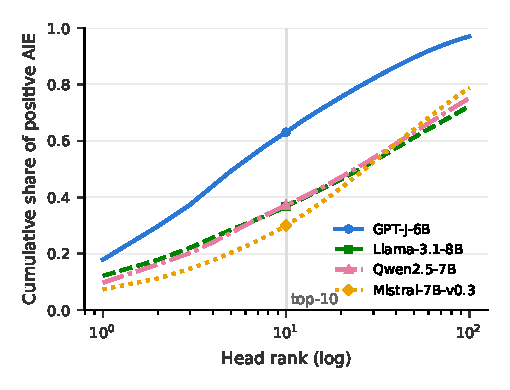
\includegraphics[width=\columnwidth]{F2_aie_concentration.pdf}
\caption{Cumulative share of positive mean AIE mass by head rank (log
scale), averaged over the six tasks. GPT-J concentrates 0.63 of its causal
task signal in the top-10 heads; all three modern models are flatter, and
Mistral-7B-v0.3 is flattest.}
\label{fig:f2}
\end{figure}

\subsection{Concentration of causal effect}
\label{sec:concentration}

The head-count results predict that the AIE distribution over heads is
flatter in Mistral than in the other models.
Table~\ref{tab:T4_aie_concentration} and Figure~\ref{fig:f2} confirm this
directly from the measured indirect effects, upstream of any FV
construction. GPT-J's top-10 heads capture 0.63 of total positive AIE mass;
all three modern models are far flatter (0.37, 0.37, 0.30), with Mistral
lowest. Mistral is also weakest in absolute terms: its largest single-head
mean AIE (0.021) is $2.5$--$6.7\times$ smaller than the other models'
(0.053--0.142).

Two readings follow. First, the original ``small set of causal heads''
picture is quantitatively GPT-J-like only for GPT-J; on modern models the
causal mass is more spread out even when the top-10 FV works (Llama and
Qwen both sit at 0.37). Second, concentration alone does not predict
transfer --- Llama and Qwen succeed at the same top-10 share where Mistral
fails; what singles out Mistral is the combination of the flattest
distribution with per-head effects several times weaker.

\begin{table}[t]
\centering
\small
\begin{tabular}{lrrrr}
\toprule
Model & \# heads & Top-10 AIE share & Top-1\% AIE share & Max per-head AIE \\
\midrule
GPT-J-6B & 448 & 0.63 & 0.44 & 0.142 \\
Llama-3.1-8B & 1024 & 0.37 & 0.37 & 0.127 \\
Qwen2.5-7B & 784 & 0.37 & 0.34 & 0.053 \\
Mistral-7B-v0.3 & 1024 & 0.30 & 0.30 & 0.021 \\
\bottomrule
\end{tabular}
\caption{T4: Concentration of causal task signal. Share of total positive mean AIE mass captured by the top-10 (and top-1% of) heads, and the largest single-head mean AIE, averaged over the six tasks.}
\label{tab:T4_aie_concentration}
\end{table}


\section{Discussion}
\label{sec:discussion}

Our results sort into one reproduction and five boundary conditions.

\paragraph{The core finding is architecture-robust.} On two of three
modern GQA models, the unchanged GPT-J recipe produces FV effects as large
as, or larger than, on GPT-J. Nothing about grouped-query attention,
larger vocabularies, or newer training pipelines is inherently hostile to
function vectors.

\paragraph{Boundary 1: english-french is a task-general failure.} The
translation FV works only on GPT-J. Two candidate contributors: (i)~French
targets are multi-token under all tokenizers involved, and our first-token
metric may under-credit partially correct continuations --- though GPT-J
succeeds under the same metric, so the metric alone cannot explain the gap;
(ii)~word-level translation may be represented differently (or more
diffusely) in models trained on far more multilingual data. Distinguishing
these requires a string-generation metric, which we flag as follow-up.

\paragraph{Boundary 2: present-past is a Llama-3.1-specific failure.}
Since the sibling morphological task singular-plural transfers on
Llama-3.1 at $+0.78$, this is not a statement about morphology but an
idiosyncrasy of how one model represents one task --- a caution against
reading any single (model, task) failure as a general claim.

\paragraph{Boundary 3: the $L/3$ rule is GPT-J-specific.} The effective
injection band drifts from $0.32\times$ depth (GPT-J) to $0.42\times$
(Llama-3.1) to $0.61\times$ (Qwen2.5). Work that hard-codes the original
layer heuristic on a new model may silently measure a much weaker effect
than the model actually supports (\S\ref{sec:layers}).

\paragraph{Boundary 4: Mistral-7B-v0.3 and the ``small set of heads''
claim.} Mistral is the strongest challenge to the original picture, and we
state it carefully. We first verified the null is not a pipeline bug; five
independent observations contradict that hypothesis
(analysis detailed in our released verification note):
(i)~the final Mistral results were produced by verified-fixed code shared
with a working model --- the same long-lived process had already executed
the previously-faulty code path successfully on Qwen2.5; (ii)~Mistral's
ICL is healthy under the identical first-token metric (10-shot accuracy
0.71--1.00 across tasks), so the model \emph{has} each task; (iii)~the
intervention demonstrably perturbs the forward pass --- at early layers
the injected FV \emph{degrades} zero-shot accuracy by up to 0.19
(present-past) and 0.42 (singular-plural); (iv)~the injection scale is not
anomalous --- Mistral's FV-to-residual-stream norm ratio (0.33) is
identical to Qwen2.5's (0.33), whose FV works; (v)~the effect recovers
smoothly and monotonically with head count (0.09 at $k{=}5$ to 0.45 at
$k{=}100$), which a broken intervention could not produce.

What remains is a property of the model, and the positive evidence points
one way: the flattest AIE distribution (top-10 share 0.30), the weakest
per-head causal effects (max 0.021), and the monotone $k$ dose-response
are all \emph{consistent with} a task representation distributed across
roughly an order of magnitude more heads than the method's top-10 default
captures. We do not claim this is the full explanation: capitalize's total
collapse ($+0.01$ against $+0.78$ to $+0.94$ on every other model) and
country-capital's non-recovery through $k{=}50$ are not explained by the
distributed account, and we flag them as open residuals
(\S\ref{sec:limitations}). The non-recovery does, however, argue against
one further artifact hypothesis --- scrambled head \emph{selection}: if
the AIE ranking were quasi-random, adding heads should recover all tasks
at broadly similar rates, not antonym alone.

\paragraph{Boundary 5: vocab-decodability of FVs does not generalize.}
\citet{todd2024function} report (their \S3.2) that decoded FV tokens lie
within the task's output space \emph{for most tasks} --- they themselves
note English--French as an exception that decodes to nonsense on GPT-J
even though its FV works, while antonym decodes to words evoking the
abstract idea of reversal. We reproduce the antonym case on GPT-J --- its
FV decodes to tokens such as \emph{`` vs''}, \emph{`` counterpart''},
\emph{`` versus''}, \emph{`` oppos-''} --- but on all three modern models
even the antonym FV decodes to noise (whitespace, punctuation, unrelated
code and multilingual fragments), \emph{including on Llama-3.1 and
Qwen2.5, whose FVs work}. Their per-task caveat thus extends to a
per-model one: on modern models, decodability fails even for the task
that decodes most cleanly on GPT-J. Because decodability does not
separate Mistral from the working modern models, we do not use it as
evidence in Boundary 4. The FV \emph{mechanism} transfers to modern
models, but vocabulary readout as a window into FVs is GPT-J-specific:
interpretability methods that validate interventions by reading them
through the unembedding would declare these working FVs broken.

\paragraph{An architectural boundary of the tooling.} Independent of any
result, the released FV code assumes
$d_{\text{head}} \times n_{\text{heads}} = d_{\text{model}}$ to reconstruct
per-head contributions from the attention output projection. Gemma-2/3
violate this and are excluded here. As decoupled head dimensions become
more common, interpretability tooling that hard-codes this identity will
silently exclude (or worse, mis-split) a growing slice of the model
population.

\section{Limitations}
\label{sec:limitations}

\textbf{Single seed, single run per cell.} All numbers come from one run
at seed 42; we report no variance. Cells with small filtered test sets
(country-capital, present-past, singular-plural: $n = 41$--$60$) carry
sampling noise of several points, and fine-grained orderings (e.g.\
non-monotonic $k$-responses in Table~\ref{tab:T3_k_ablation}) should be
read accordingly. The large qualitative gaps (transfer vs.\ null) are far
outside this noise: the worst-case binomial 95\% confidence half-width at
$n{=}41$ ($p{=}0.5$) is $\pm 0.15$, well below the transfer effects of
$+0.33$ to $+0.94$ against nulls of $\le +0.07$.
\textbf{First-token top-1 metric.} Inherited from the original evaluation;
it under-credits multi-token answers, which is most acute for
english-french. Our conclusion there is robust to the direction of this
bias only because GPT-J succeeds under the same metric; a
string-generation metric would strengthen it.
\textbf{Best-layer selection.} $\ell^*$ maximizes effect on the same
filtered test set it is evaluated on --- an oracle over 28--32 layers.
This inflates all models equally and favors finding transfer, making the
null and near-null cells conservative.
\textbf{Unexplained residuals.} The distributed-representation account of
Mistral does not explain capitalize's total collapse or country-capital's
non-recovery through $k{=}50$; probing these (e.g.\ $k > 100$, per-layer
FV composition) is future work.
\textbf{Coverage.} Six of the original ${\sim}40$ tasks; three modern
models in the 7--8B range, base checkpoints only; filtered evaluation sets
condition on 10-shot ICL success. Findings may not extend to larger
scales, instruction-tuned models, or the task long tail.

% TODO-CHECK(user): add an Acknowledgments section for camera-ready (omitted
% entirely in review mode to preserve anonymity).

\bibliography{refs}

\appendix

\section{Per-task layer sweeps}
\label{app:facets}

\begin{figure*}[t]
\centering
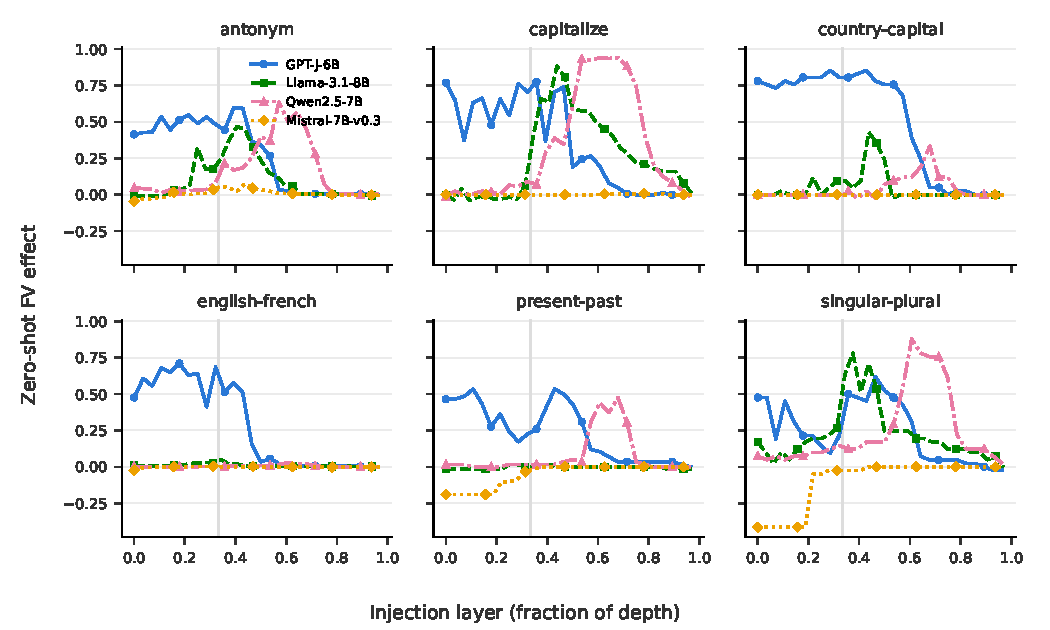
\includegraphics[width=\textwidth]{F1b_layer_sweep_facets.pdf}
\caption{Per-task FV effect vs.\ injection depth (top-10 heads), the
disaggregation of Figure~\ref{fig:f1}. The english-french panel shows the
task-general failure on all modern models (Boundary 1); present-past shows
the Llama-3.1-specific failure (Boundary 2); the rightward shift of the
Qwen2.5 curves is Boundary 3.}
\label{fig:f1b}
\end{figure*}

\end{document}
